In this chapter, we will discuss the performance of our approach towards neural networks.
By performance, we mean the ability of our approach to improve the accuracy of a pre-trained model and how much our approach can reduce the loss of a pre-trained model.
We will explore various options available through our approach to the elicit optimal results.
To achieve this, the evaluation will be based on the following research questions:
\begin{enumerate}
    \item[]\textbf{RQ1: Impact of Training on Mutated Models} How does training a mutated pre-trained model impact its performance metrics?
    \item[]\textbf{RQ2: Effects of Mutation Without Training} What is the effect on performance metrics when a pre-trained model is mutated without further training?
    \item[]\textbf{RQ3: Effects of the extend of pre Training} What is the effect on performance metrics, depending on how many epochs the model is pre-trained?
    \item[]\textbf{RQ4: Training Dataset Size and Approach Performance} What is the impact of the size of the training dataset on the approach's effectiveness?
    \item[]\textbf{RQ5: Influence of Suspiciousness Measures} How do different suspiciousness measures influence the outcomes of the experiments?
    \item[]\textbf{RQ6: CNN vs. DNN Architectural Efficiency} Which architecture yields better results for our approach: CNN or DNN?
    \item[]\textbf{RQ7: Offset Variations in Loss and Accuracy} How do variations in offset for loss and accuracy affect the approach's performance?
    \item[]\textbf{RQ8: Break Conditions and Algorithm Performance} What is the effect of different break conditions on the efficiency and effectiveness of the algorithm?
    \item[]\textbf{RQ9: Contributions of Different Mutation Functions} How do different mutation functions contribute to the model's performance with our Algorithm?
\end{enumerate}
\section{Setup}\label{sec:setup}

We evaluated our approach on a Workstation consisting of an AMD Ryzen 9 3900X 12-Core Processor 4,6 GHz, with 32 GB of RAM and an NVIDIA GeForce RTX 4070Ti GPU with 12 GB of VRAM and 7680 CUDA Cores.
The setup is running Ubuntu release 22.04, running with Windows Subsystem for Linux, on Microsoft Windows 11 Pro, we use it because since version 2.11\cite{noauthor_build_2023} TensorFlow doesn't support GPU acceleration natively any more.
Regarding the Software, we are using Python version 3.10.12 and using TensorFlow version 2.14.1, with CUDA version 12.3.

\subsection{Architecture}\label{subsec:architecture}
We are using the Fashion-MNIST dataset\cite{xiao_fashion-mnist_2017} for our experiments, which consists of 60,000 training images and 10,000 test images, each of size 28×28 pixels, with 10 classes.
For the evaluation we haven't used not only the whole, but also a half and a quarter of the training data, which are derived from the original training data, by using Scikit-learn's\cite{pedregosa_scikit-learn_2011} \texttt{train\_test\_split} function, with a test size of 0.5 and 0.75 respectively.

We used 2 DNNs and 2 CNNs, in the following table \ref{tab:archi} a plain number describes the number of neurons in a dense layer. $CL$ describes a combination of a convolutional layer with a stride of $(1,1)$ and a kernel size of $(3,3)$ and a pooling layer with a pool size of $(2,2)$. We used.
Adam as our optimizer with a learning rate of 0.001.

The models were selected for their small size and ability to accommodate both deep neural networks and convolutional neural networks.
This was done to save time and allow for the evaluation of as many parameters as possible within the time frame of this thesis.
% Please add the following required packages to your document preamble:
% \usepackage{multirow}
% \usepackage{lscape}
% Please add the following required packages to your document preamble:
% \usepackage{multirow}
\begin{table}[htbp]
    \centering
    \caption{Overview of Neural Network Architectures used for evaluation}
    \begin{tabular}{|c|c|c|}
        \hline
        Model Name            & Mod. Param.         & Architecture                 \\ \hline
        \multirow{2}{*}{DNN1} & \multirow{2}{*}{16} & \multirow{2}{*}{$<16>$}      \\
        &                     &                              \\ \hline
        \multirow{2}{*}{DNN2} & \multirow{2}{*}{64} & \multirow{2}{*}{$<4x16>$}    \\
        &                     &                              \\ \hline
        \multirow{2}{*}{CNN1} & \multirow{2}{*}{12} & \multirow{2}{*}{$<CL,4>$}    \\
        &                     &                              \\ \hline
        \multirow{2}{*}{CNN2} & \multirow{2}{*}{20} & \multirow{2}{*}{$<CL,CL,4>$} \\
        &                     &                              \\ \hline
    \end{tabular}
    \label{tab:archi}
\end{table}
\begin{table}[htbp]
    \centering
    \caption{Results of the initial Training of the different models}
    \begin{tabular}{|cc|ccc|ccc|}
        \hline
        \multicolumn{2}{|c|}{Model} & \multicolumn{3}{c|}{Accuracy} & \multicolumn{3}{c|}{Loss} \\ \hline
        \multicolumn{1}{|c|}{Name}                  & Init. Epochs & \multicolumn{1}{c|}{Full}    & \multicolumn{1}{c|}{Half}    & Quarter & \multicolumn{1}{c|}{Full}    & \multicolumn{1}{c|}{Half}     & Quarter  \\ \hline
        \multicolumn{1}{|c|}{\multirow{2}{*}{DNN1}} & 1              & \multicolumn{1}{c|}{82.84\%} & \multicolumn{1}{c|}{81.49\%} & 78.65\% & \multicolumn{1}{c|}{49.11\%} & \multicolumn{1}{c|}{53.46\%}  & 62.00\%  \\ \cline{2-8}
        \multicolumn{1}{|c|}{}                      & 6              & \multicolumn{1}{c|}{84.23\%} & \multicolumn{1}{c|}{83.76\%} & 83.57\% & \multicolumn{1}{c|}{44.42\%} & \multicolumn{1}{c|}{44.48\%}  & 46.94\%  \\ \hline
        \multicolumn{1}{|c|}{\multirow{2}{*}{DNN2}} & 1              & \multicolumn{1}{c|}{80.46\%} & \multicolumn{1}{c|}{79.20\%} & 75.97\% & \multicolumn{1}{c|}{54.05\%} & \multicolumn{1}{c|}{57.90\%}  & 66.21\%  \\ \cline{2-8}
        \multicolumn{1}{|c|}{}                      & 6              & \multicolumn{1}{c|}{83.52\%} & \multicolumn{1}{c|}{83.04\%} & 82.74\% & \multicolumn{1}{c|}{44.23\%} & \multicolumn{1}{c|}{46.79\%}  & 48.88\%  \\ \hline
        \multicolumn{1}{|c|}{\multirow{2}{*}{CNN1}} & 1              & \multicolumn{1}{c|}{74.34\%} & \multicolumn{1}{c|}{77.31\%} & 42.62\% & \multicolumn{1}{c|}{72.88\%} & \multicolumn{1}{c|}{66.83\%}  & 147.63\% \\ \cline{2-8}
        \multicolumn{1}{|c|}{}                      & 6              & \multicolumn{1}{c|}{83.69\%} & \multicolumn{1}{c|}{82.14\%} & 61.06\% & \multicolumn{1}{c|}{48.44\%} & \multicolumn{1}{c|}{47.35\%}  & 95.61\%  \\ \hline
        \multicolumn{1}{|c|}{\multirow{2}{*}{CNN2}} & 1              & \multicolumn{1}{c|}{70.49\%} & \multicolumn{1}{c|}{54.52\%} & 63.20\% & \multicolumn{1}{c|}{80.13\%} & \multicolumn{1}{c|}{111.68\%} & 100.31\% \\ \cline{2-8}
        \multicolumn{1}{|c|}{}                      & 6              & \multicolumn{1}{c|}{78.43\%} & \multicolumn{1}{c|}{77.37\%} & 74.56\% & \multicolumn{1}{c|}{60.28\%} & \multicolumn{1}{c|}{59.29\%}  & 65.74\%  \\ \hline
    \end{tabular}
    \label{tab:results}
\end{table}
\subsection{Parameters}\label{subsec:parameters}
Fo our evaluation we used the following parameters:
\begin{enumerate}
    \item[]\textbf{Similarity coefficient:} tarantula, dstar with value 3, ochiai and random
    \item[]\textbf{Mutation functions:} \texttt{modify\_weight\_one\_random\_gauss,\\ modify\_weight\_all\_random\_gauss, modify\_bias, modify\_bias\_random\_gauss, modify\_all\_weights, modify\_all\_weights\_by\_scalar,\\modify\_all\_weights\_by\_scalar\_random\_gauss,\\modify\_weight\_all\_random\_by\_scalar\_gauss}
    \item[]\textbf{Break conditions:} loss, accuracy, loss and accuracy, loss or accuracy
    \item[]\textbf{Loss offset:} 0.005, 0
    \item[]\textbf{Accuracy offset:} 0.01, 0
    \item[]\textbf{Loss and accuracy regression:} True for all runs
    \item[]\textbf{Values:} -1, -0.5, 0, 0.5, 1\\ \textit{0 just for value assignment, basically a deletation of a neuron}
    \item[]\textbf{Sigma for random:} 0.5, 1
\end{enumerate}
We chose these parameters to evaluate the impact of different mutation functions, suspiciousness measures, and break conditions on the performance of our approach.
Our main objective was to cover a large area of the possible parameter space to evaluate the performance of our approach, with as little parameters as possible.
\section{Results}\label{sec:results}
This section will present the findings of our experiments.
The two measures we used to compare our methods are the change in loss and the change in accuracy.
The change is based on the benchmark, which is the model without any mutations.
For the further trained models, we compared the comparison model with the respective epoch of out algorithm.
For example, the results of the 1st epoch of our algorithm for a model pre-trained for 1 epoch is compared the model trained for 2 epochs, for 6 epochs it would be compared to the model trained for 7 epochs.
For the models without training, we always compared to the base accuracy and loss seen in the table \ref{tab:results}.


\subsection{Impact of Training on Mutated Models}\label{subsec:impact-of-training-on-mutated-models}
Our models \ref{fig:loss-accuracy-training} show slightly better loss and accuracy than the benchmark during training.
For the first four epochs, the loss and accuracy of the models are significantly better than the benchmark.
We see an improvement in the median for the accuracy of 1.75\% and for the loss of 3--4\%.
Afterwards, we see a decrease of the median to the baseline of 1.
After the 11th epoch, we see a drop of the median below the baseline.
This holds also true for the loss, where we see the same drop after the 11th epoch.

For some epochs we can see an improvement to 2.5\% for the accuracy to an extreme of 7.5\%.
For the loss, we see an 12\% improvement to an extreme of 40\%.
We would attribute this to the mutation of the model and the breakage of the algorithm, as we can see in the figure \ref{fig:decay_training}.

\begin{figure}
    \centering
    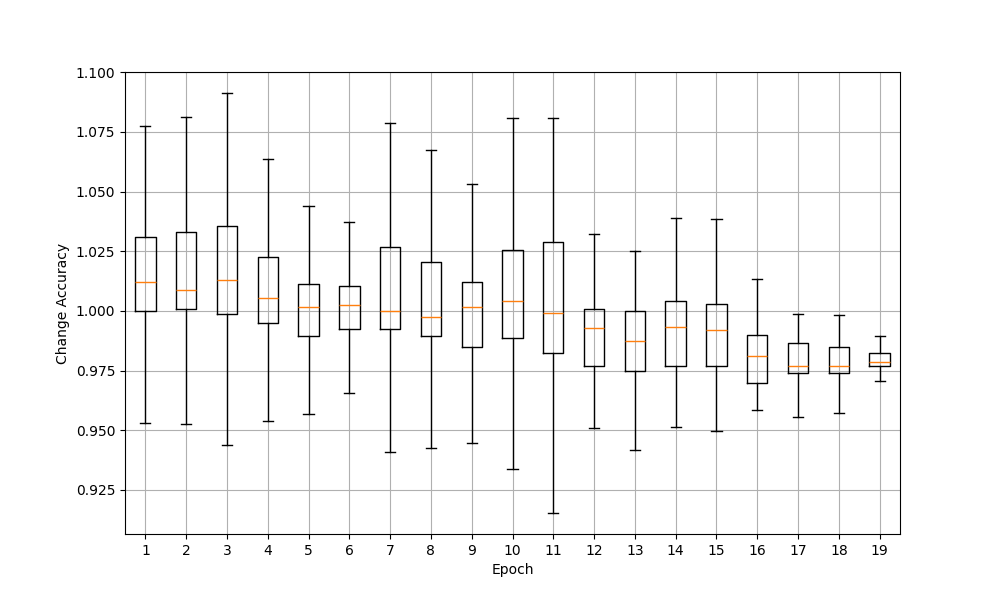
\includegraphics[width=\textwidth]{plots/Trained_Change_Acc.png}
    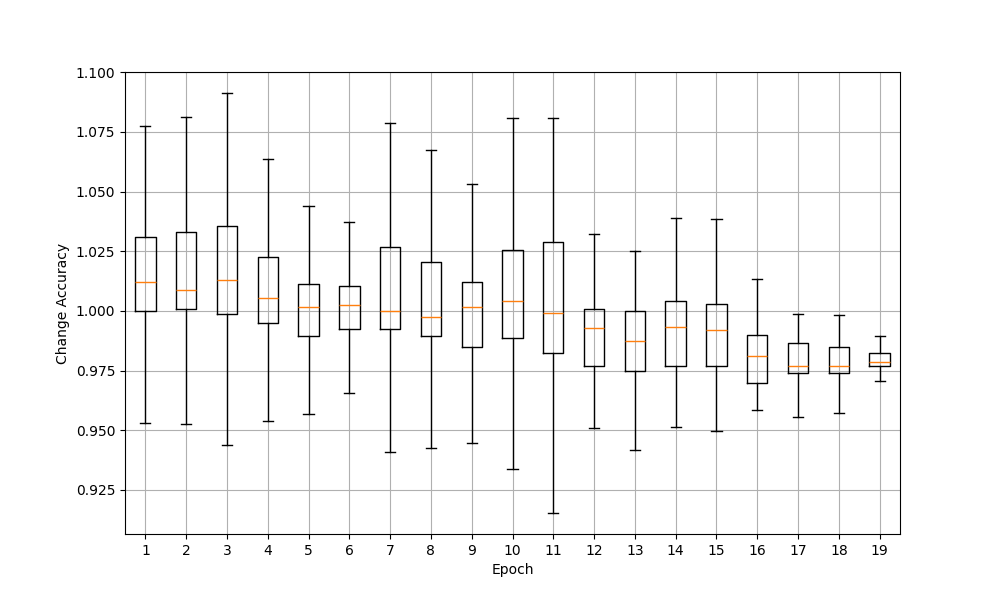
\includegraphics[width=\textwidth]{plots/Trained_Change_Loss.png}
    \caption{Loss and accuracy of the models, with training}
    \label{fig:loss-accuracy-training}
\end{figure}
\begin{figure}
    \centering
    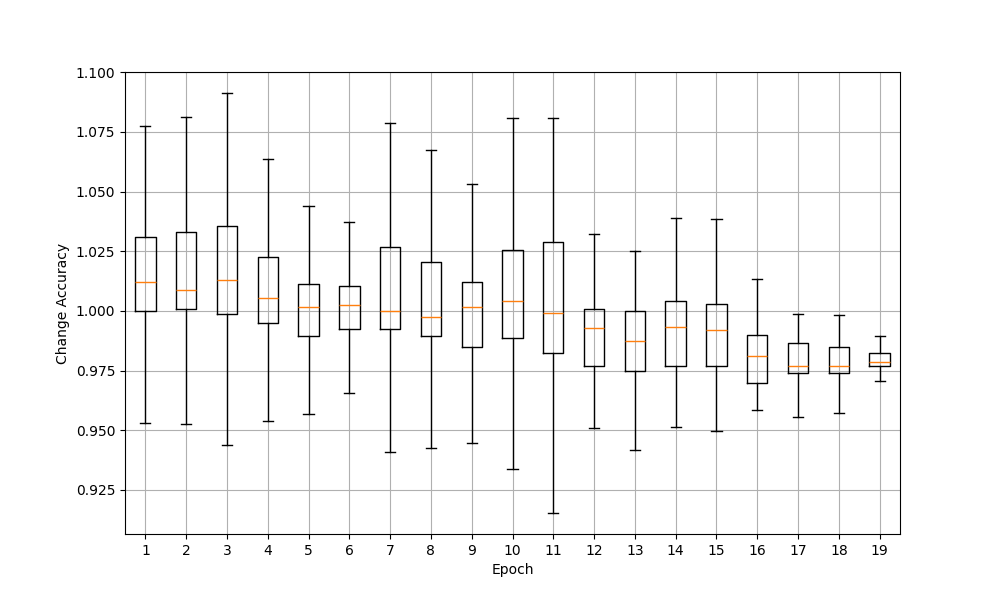
\includegraphics[width=\textwidth]{plots/Trained_Points_perEpoch.png}
    \caption{Decay of data points, per epoch, with training}
    \label{fig:decay_training}
\end{figure}
\subsection{Effects of Mutation Without Training}\label{subsec:effects-of-mutation-without-training}
As you can see in the figure \ref{fig:loss-accuracy-Notraining}, the models without training show a significant improvement in accuracy and loss during the first three epochs.
But we see only a median that isn't significantly better than the baseline of 1, for both loss and accuracy.
We see a in crease for the extremes stepwise, for each of the first 3 epochs, till we reach an improvement of 25\%, but on the other hand a decrease of -17\% on the other extreme.
The same for the loss, where we see an improvement of 45\% to a decrease of -50\%.

The three steps we are seeing, can be attributed to the comparison to only the 1st epoch, or 6th epoch respectively, so we are summing up any improvement of the model.
The reason for the sharp drop we see in the figure \ref{fig:decay_Notraining}, we would attribute to to the increasing damage we are doing to the model, as we are not training it in between the mutations.
\begin{figure}
    \centering
    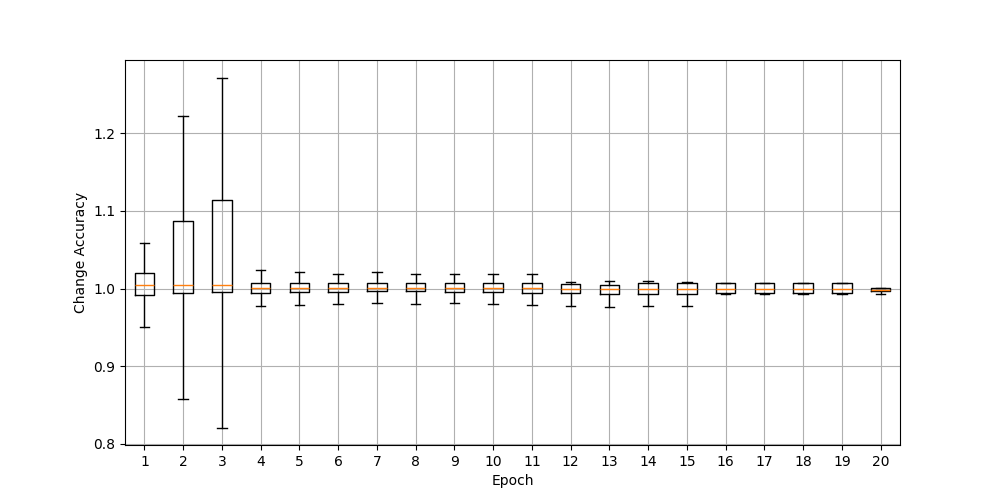
\includegraphics[width=\textwidth]{plots/NotTrained_Change_Acc.png}
    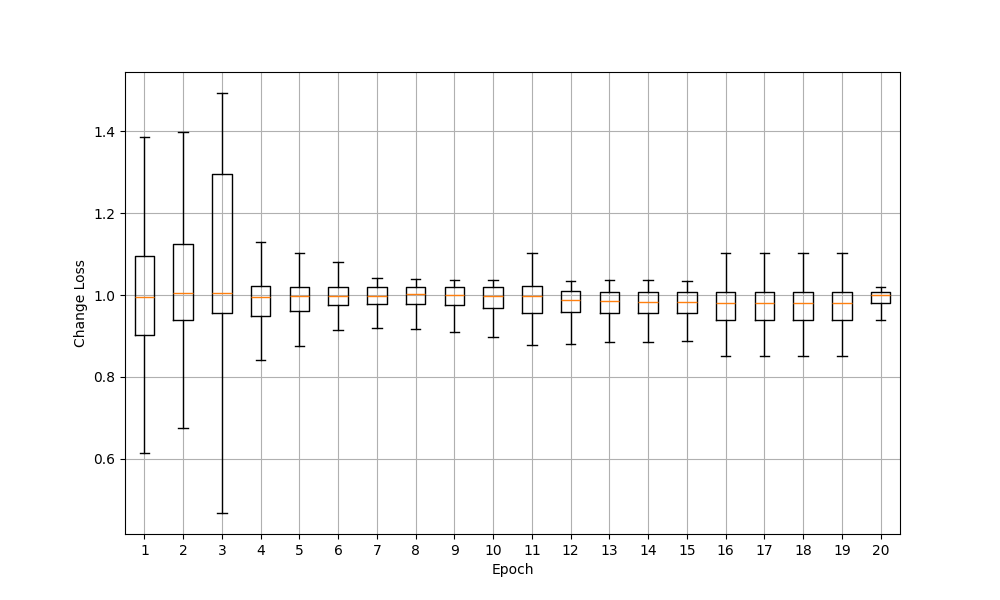
\includegraphics[width=\textwidth]{plots/NotTrained_Change_Loss.png}
    \caption{Loss and accuracy of the models, without training}
    \label{fig:loss-accuracy-Notraining}
\end{figure}
\begin{figure}
    \centering
    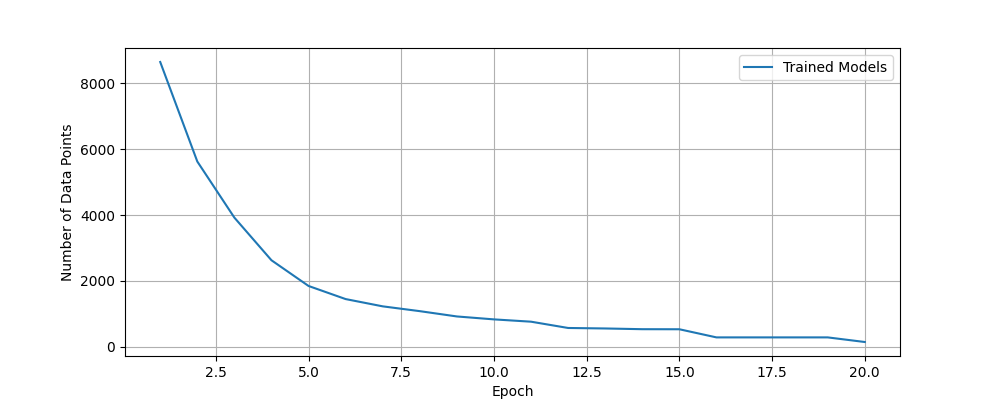
\includegraphics[width=\textwidth]{plots/NotTrained_Points_perEpoch.png}
    \caption{Decay of data points, per epoch, without training}
    \label{fig:decay_Notraining}
\end{figure}
\subsection{Effects of the extend of pre-Training}\label{subsec:effects-of-the-extend-of-pre-training}
As we can see in the figure \ref{fig:initial-epochs-notraining}, the models with 1 initial epoch show the largest potential for improvements.
While for the not trained runs, the median for loss and acurracy is not significantly better than the baseline, we can see a significant improvement for the extremes.
With a maximum improvement of 25\% for the accuracy and 45\% for the loss, for the 1st epoch.
But a decrease of up to -40\% for the accuracy and -70\% for the loss.
For the 6 initial epochs, we see a lower derivation.

For the trained runs, that can be seen in figure \ref{fig:initial-epochs-training},we see a smaller improvement over all, which is in line with the results of the previous two subsections.
But here we also see a better result for the 1 initial epoch, than for the 6 initial epochs.
But also a larger derivation for 1 initial epoch, than for the 6 initial epochs.

We would guess that the reason tHat the 1 initial epoch has more room for improvement, then the 6 initial epoch.
As we can see in the table \ref{tab:results} that the accuracy and loss of the 6 initial epochs is already better than the 1 initial epoch, at the beginning.
\begin{figure}
    \begin{subfigure}{0.5\textwidth}
        \centering
        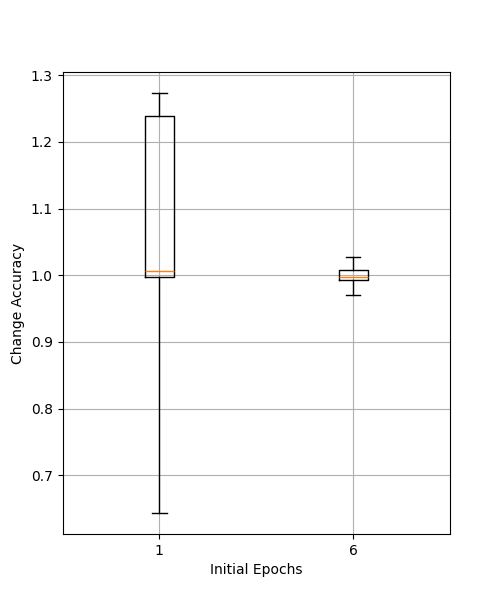
\includegraphics[width=0.95\textwidth]{plots/InitEpoch_NotTrained_accuracy.png}
    \end{subfigure}
    \begin{subfigure}{0.5\textwidth}
        \centering
        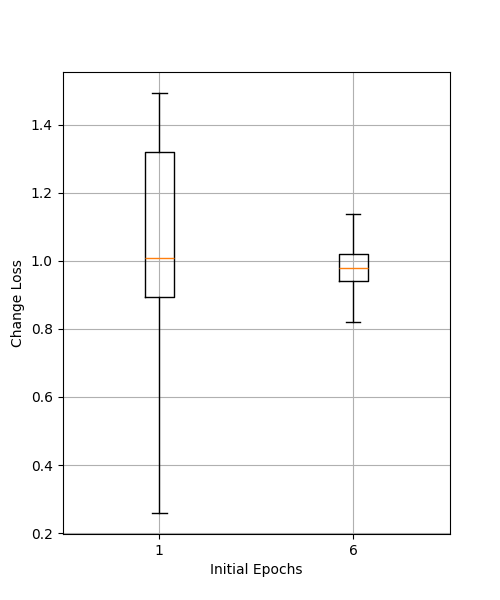
\includegraphics[width=0.95\textwidth]{plots/InitEpoch_NotTrained_loss.png}
    \end{subfigure}
    \caption{Loss and accuracy, without training, with different initial epochs}
    \label{fig:initial-epochs-notraining}
\end{figure}
\begin{figure}
    \begin{subfigure}{0.5\textwidth}
        \centering
        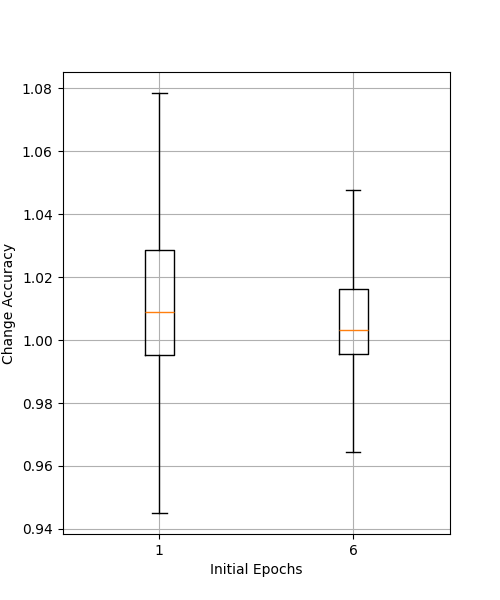
\includegraphics[width=0.95\textwidth]{plots/InitEpoch_Trained_accuracy.png}
    \end{subfigure}
    \begin{subfigure}{0.5\textwidth}
        \centering
        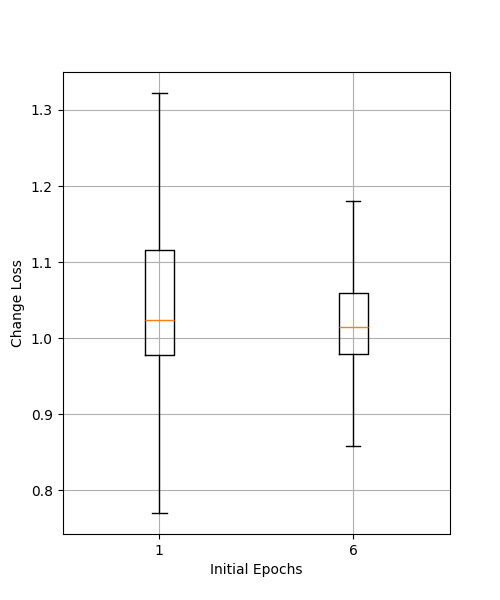
\includegraphics[width=0.95\textwidth]{plots/InitEpoch_Trained_loss.png}
    \end{subfigure}
    \caption{Loss and accuracy, with training, with different initial epochs}
    \label{fig:initial-epochs-training}
\end{figure}
\subsection{Training Dataset Size and Model Performance}\label{subsec:training-dataset-size-and-model-performance}
As you can see in the figure \ref{fig:dataset-size-notraining}, the dataset size doesn't have a significant impact on the loss and accuracy of the models without training, for the full and half dataset.
While we see a improvement for the full and half dataset, for the accuracy of often up to 25\% and for the loss a slight different result with 50\% and 30\% respectively.
For the quarter dataset we see a more negative result, while a improvement is still possible, we even see the 3rd quartile just slightly above the baseline.
And the rest all below the baseline, so roughly only a quarter of the models are better than the baseline.

For the trained runs, that can be seen in the figure \ref{fig:dataset-size-training}, we see a larger difference between the full and half dataset.
With the full dataset, we see an improvement of up to 25\% for the accuracy and 95\% for the loss.
We even see the 1st quartile above the baseline, so three quarters of the models are better than the baseline.
This holds also true for the half dataset, where we see an improvement of up to 7.5\% for the accuracy and a bit more than 25\% for the loss.
Here also the quarter dataset is the worst, with only half of the models better than the baseline.
And even that at most for 5\% for the accuracy and around 10\% for the loss.
\begin{figure}
    \begin{subfigure}{0.5\textwidth}
        \centering
        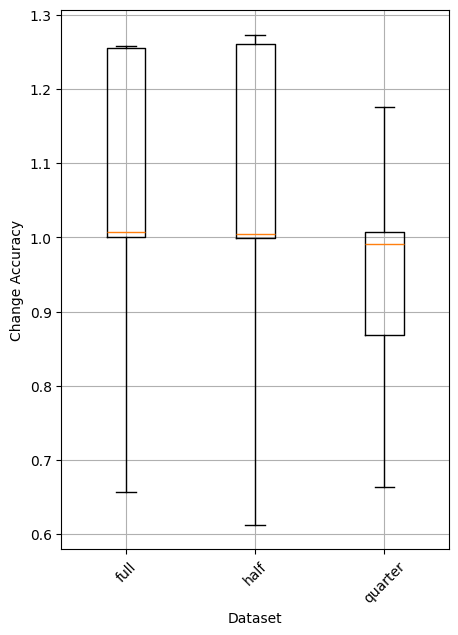
\includegraphics[width=0.95\textwidth]{plots/Dataset_NotTrained_accuracy.png}
    \end{subfigure}
    \begin{subfigure}{0.5\textwidth}
        \centering
        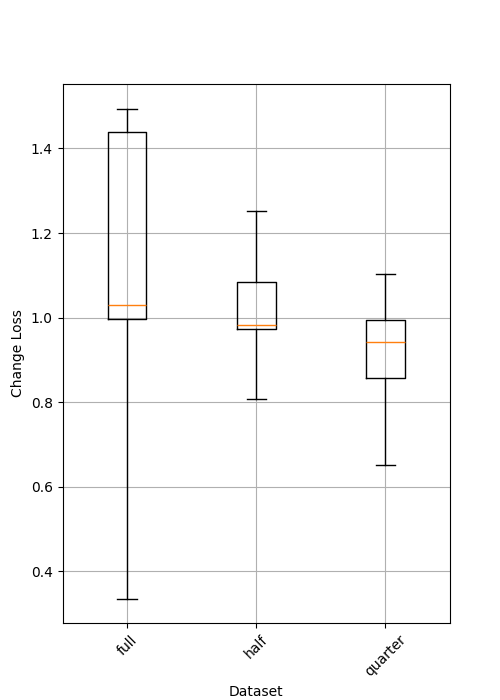
\includegraphics[width=0.95\textwidth]{plots/Dataset_NotTrained_loss.png}
    \end{subfigure}
    \caption{Loss and accuracy, without training, with different dataset sizes}
    \label{fig:dataset-size-notraining}
\end{figure}
\begin{figure}
    \begin{subfigure}{0.5\textwidth}
        \centering
        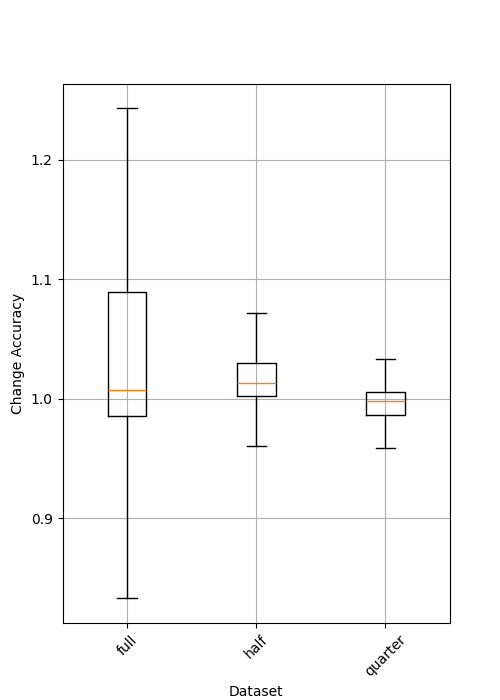
\includegraphics[width=0.95\textwidth]{plots/Dataset_Trained_accuracy.png}
    \end{subfigure}
    \begin{subfigure}{0.5\textwidth}
        \centering
        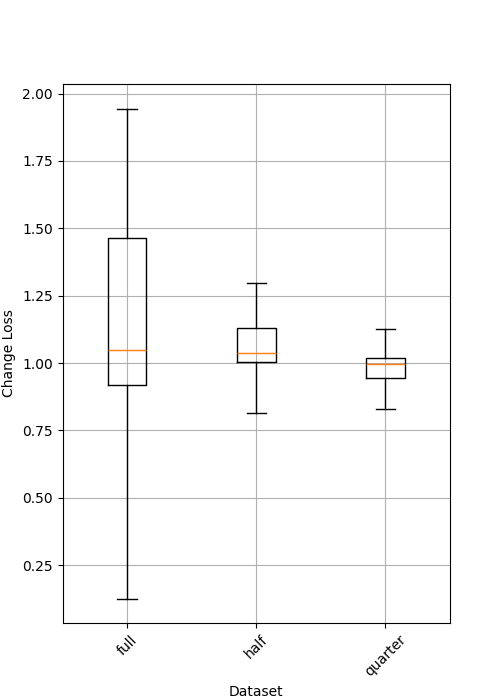
\includegraphics[width=0.95\textwidth]{plots/Dataset_Trained_loss.png}
    \end{subfigure}
    \caption{Loss and accuracy, with training, with different dataset sizes}
    \label{fig:dataset-size-training}
\end{figure}
\subsection{Influence of Suspiciousness Measures}\label{subsec:influence-of-suspiciousness-measures}
For both trained, as seen in the figure \ref{fig:suspiciousness-measures-training}, and untrained runs, as seen in the figure \ref{fig:suspiciousness-measures-notraining}, Tarantula appears to be the most promising measure of suspiciousness.
Three quarters of the models are better than the baseline, with an improvement of up to 25\% for the accuracy and 30\% for the loss, for the not trained runs and 22.5\% for the accuracy and 90\% for the loss, for the trained runs.
Ochiai seems also promising, but in contrast to Tarantula, we the third quartile is mostly below the median of tarantula, for untrained runs.
Dstar is the worst performing of the three measures, but still positive with a median slightly above the baseline, for the untrained runs.
Random performs the worst, as expected.
For the trained runs, while we see the improvements, as earlier mentioned, with tarantula, we see no specific improvement for the other measures.
All of them having a median near the baseline, and just a slightly different derivation and both sides of the baseline.
\begin{figure}
    \begin{subfigure}{0.5\textwidth}
        \centering
        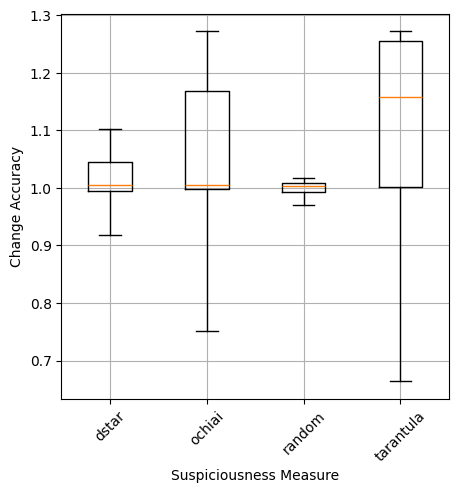
\includegraphics[width=0.95\textwidth]{plots/Meassure_NotTrained_accuracy.png}
    \end{subfigure}
    \begin{subfigure}{0.5\textwidth}
        \centering
        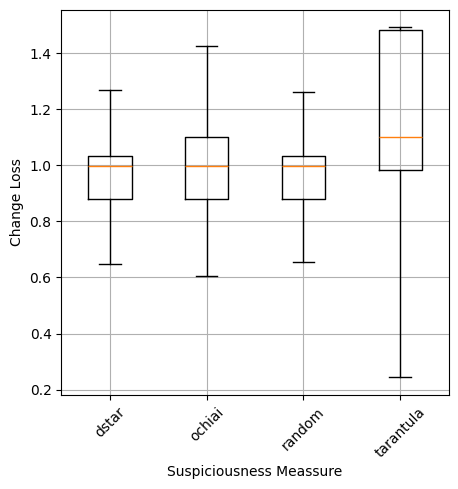
\includegraphics[width=0.95\textwidth]{plots/Meassure_NotTrained_loss.png}
    \end{subfigure}
    \caption{Loss and accuracy, without training, with different suspiciousness measures}
    \label{fig:suspiciousness-measures-notraining}
\end{figure}
\begin{figure}
    \begin{subfigure}{0.5\textwidth}
        \centering
        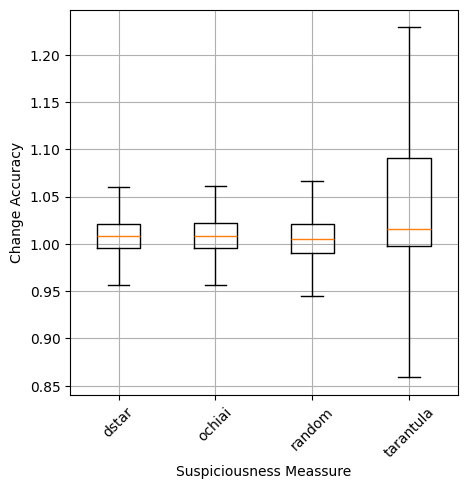
\includegraphics[width=0.95\textwidth]{plots/Meassure_Trained_accuracy.png}
    \end{subfigure}
    \begin{subfigure}{0.5\textwidth}
        \centering
        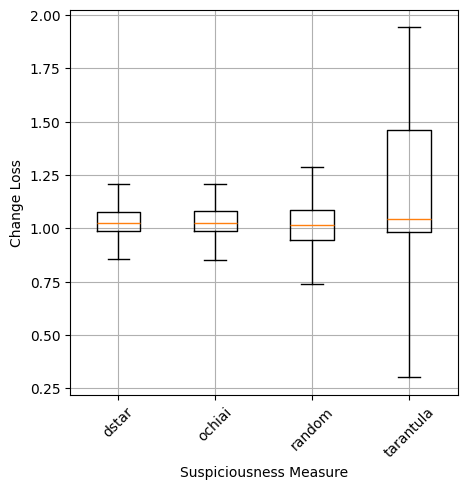
\includegraphics[width=0.95\textwidth]{plots/Meassure_Trained_loss.png}
    \end{subfigure}
    \caption{Loss and accuracy, with training, with different suspiciousness measures}
    \label{fig:suspiciousness-measures-training}
\end{figure}
\subsection{CNN vs. DNN Architectural Efficiency}\label{subsec:cnn-vs.-dnn-architectural-efficiency}
For both the trained \ref{fig:architecture-notraining} and untrained \ref{fig:architecture-training} runs, CNN1 appears to be the most promising architecture, while CNN2 shows promise for untrained runs in terms of accuracy but performs poorly in terms of loss.
For both trained and non-trained runs, the deep neural networks are not performing better than the baseline.
CNN2 is underperforming in the trained runs.
\begin{figure}
    \begin{subfigure}{0.5\textwidth}
        \centering
        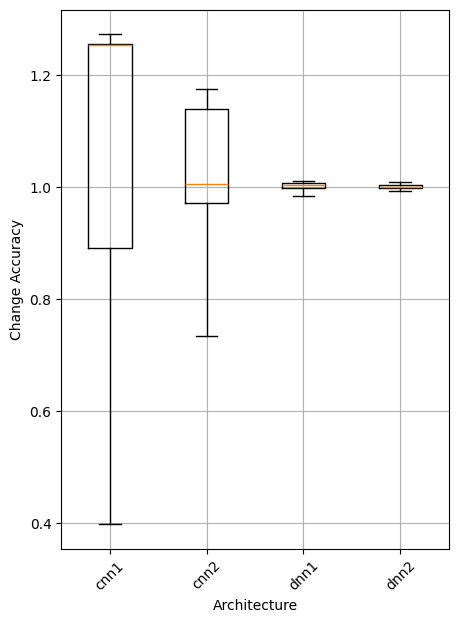
\includegraphics[width=0.95\textwidth]{plots/Architecture_NotTrained_accuracy.png}
    \end{subfigure}
    \begin{subfigure}{0.5\textwidth}
        \centering
        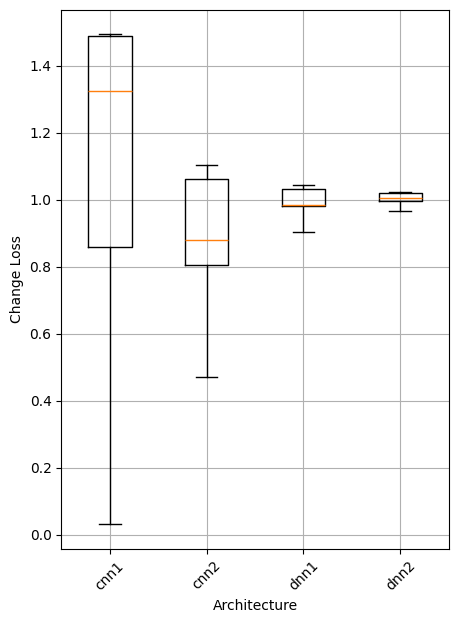
\includegraphics[width=0.95\textwidth]{plots/Architecture_NotTrained_loss.png}
    \end{subfigure}
    \caption{Loss and accuracy, without training, with different architectures}
    \label{fig:architecture-notraining}
\end{figure}
\begin{figure}
    \begin{subfigure}{0.5\textwidth}
        \centering
        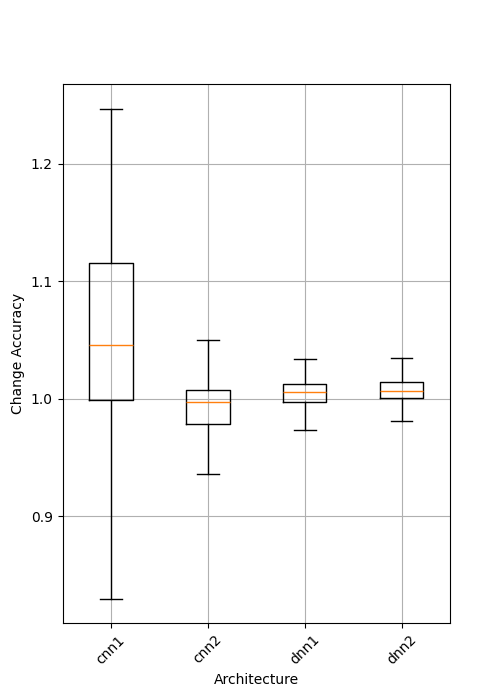
\includegraphics[width=0.95\textwidth]{plots/Architecture_Trained_accuracy.png}
    \end{subfigure}
    \begin{subfigure}{0.5\textwidth}
        \centering
        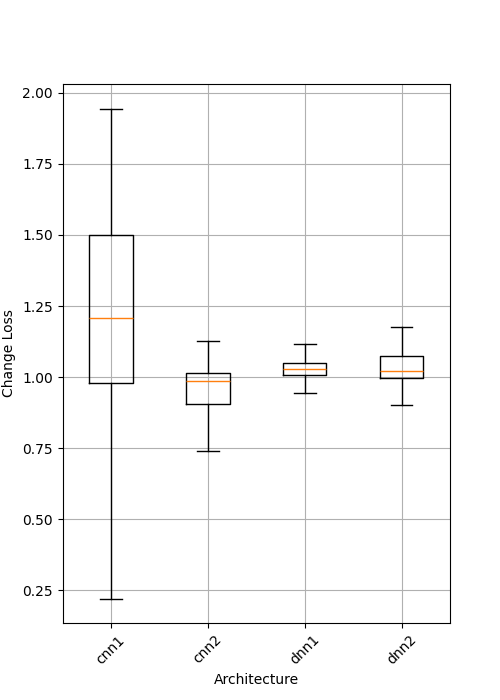
\includegraphics[width=0.95\textwidth]{plots/Architecture_Trained_loss.png}
    \end{subfigure}
    \caption{Loss and accuracy, with training, with different architectures}
    \label{fig:architecture-training}
\end{figure}
\subsection{Offset Variations in Loss and Accuracy}\label{subsec:offset-variations-in-loss-and-accuracy}
Although the median change with and without the offset is similar \ref{fig:offset-training}\ref{fig:offset-notraining}, it is important to note that the upper quartile of the categories uses the offset, as indicated by the data.
This suggests that an offset ultimately produces a better result.
\begin{figure}
    \begin{subfigure}{0.5\textwidth}
        \centering
        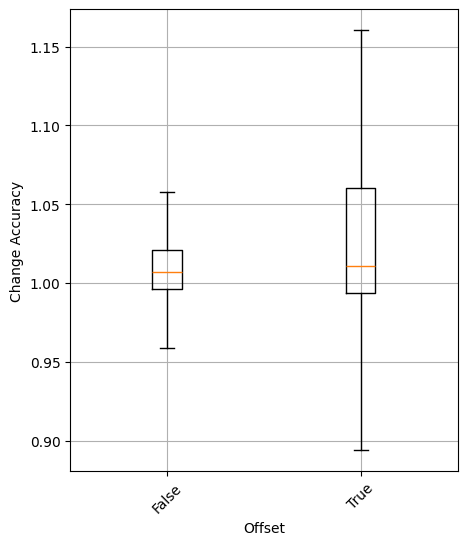
\includegraphics[width=0.95\textwidth]{plots/Offset_Trained_accuracy.png}
    \end{subfigure}
    \begin{subfigure}{0.5\textwidth}
        \centering
        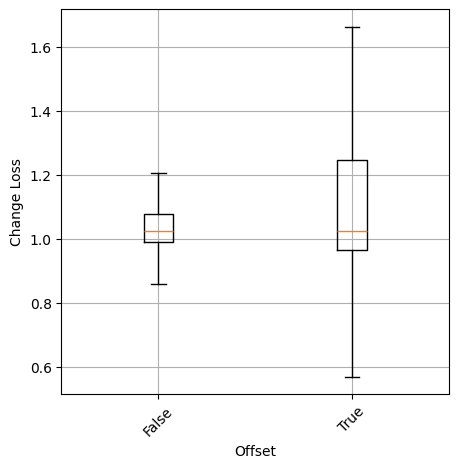
\includegraphics[width=0.95\textwidth]{plots/Offset_Trained_loss.png}
    \end{subfigure}
    \caption{Loss and accuracy, with training, with offsets or not}
    \label{fig:offset-training}
\end{figure}
\begin{figure}
    \begin{subfigure}{0.5\textwidth}
        \centering
        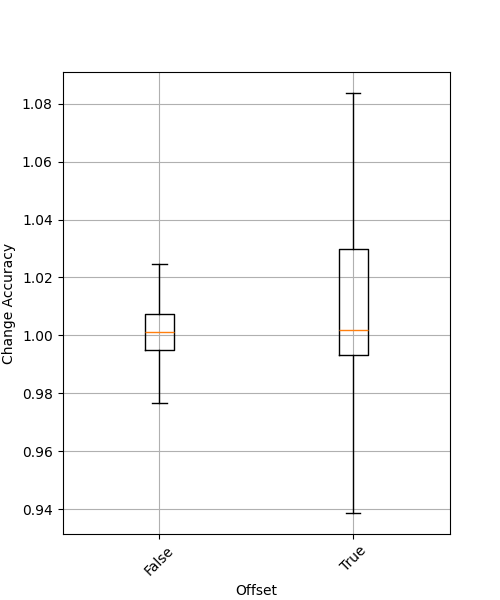
\includegraphics[width=0.95\textwidth]{plots/Offset_NotTrained_accuracy.png}
    \end{subfigure}
    \begin{subfigure}{0.5\textwidth}
        \centering
        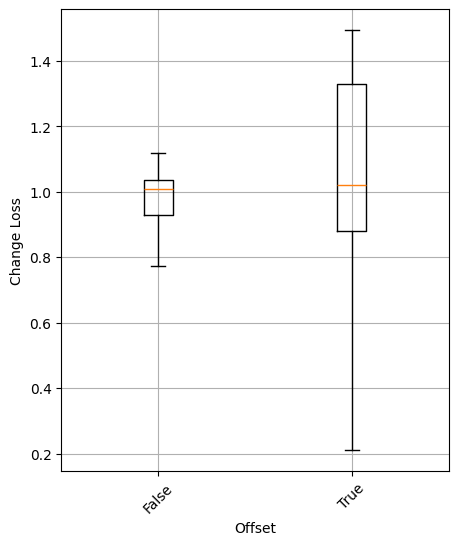
\includegraphics[width=0.95\textwidth]{plots/Offset_NotTrained_loss.png}
    \end{subfigure}
    \caption{Loss and accuracy, without training, with offsets or not}
    \label{fig:offset-notraining}
\end{figure}
\subsection{Break Conditions and Algorithm Performance}\label{subsec:break-conditions-and-algorithm-performance}
There were no significant differences observed \ref{fig:break-conditions-training} among the four options for the different break conditions.
However, some differences were noted in the samples that were not trained \ref{fig:break-conditions-notraining} during the execution of our algorithms.
In terms of accuracy, the most promising comparison appears to be between Accuracy and Loss and Accuracy.
Loss, on the other hand, seems to be neutral.
While Loss or Accuracy still results in a small improvement, it is not as significant as the first two.
For the loss also Accuracy and Loss and Accuracy seem to be the most promising, while Loss and Loss or Accuracy are rather neutral toward worsening.
\begin{figure}
    \begin{subfigure}{0.5\textwidth}
        \centering
        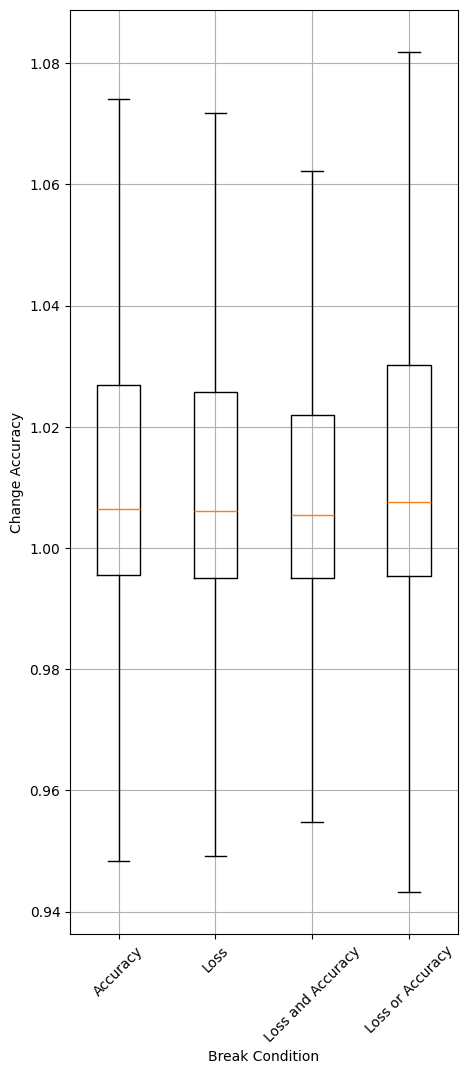
\includegraphics[width=0.95\textwidth]{plots/BreakCondition_Trained_accuracy.png}
    \end{subfigure}
    \begin{subfigure}{0.5\textwidth}
        \centering
        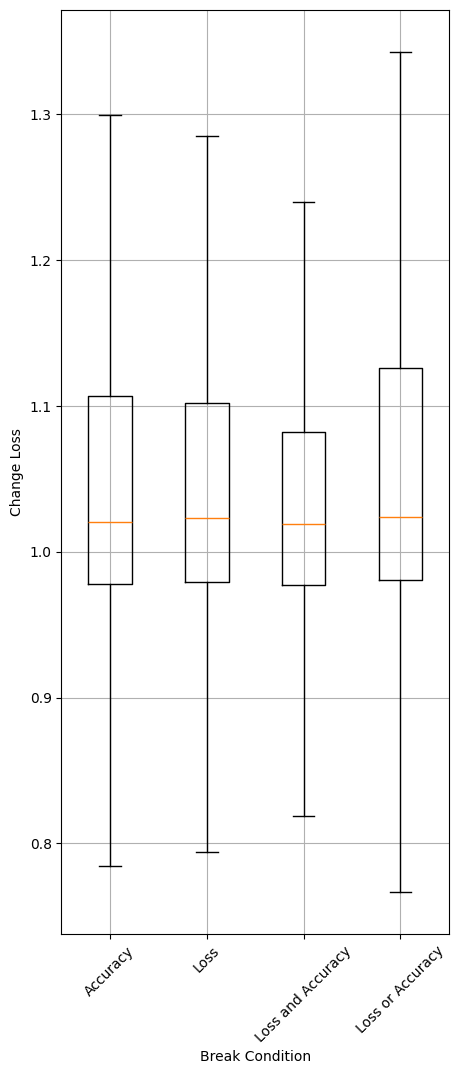
\includegraphics[width=0.95\textwidth]{plots/BreakCondition_Trained_loss.png}
    \end{subfigure}
    \caption{Loss and accuracy, with training, with different break conditions}
    \label{fig:break-conditions-training}
\end{figure}
\begin{figure}
    \begin{subfigure}{0.5\textwidth}
        \centering
        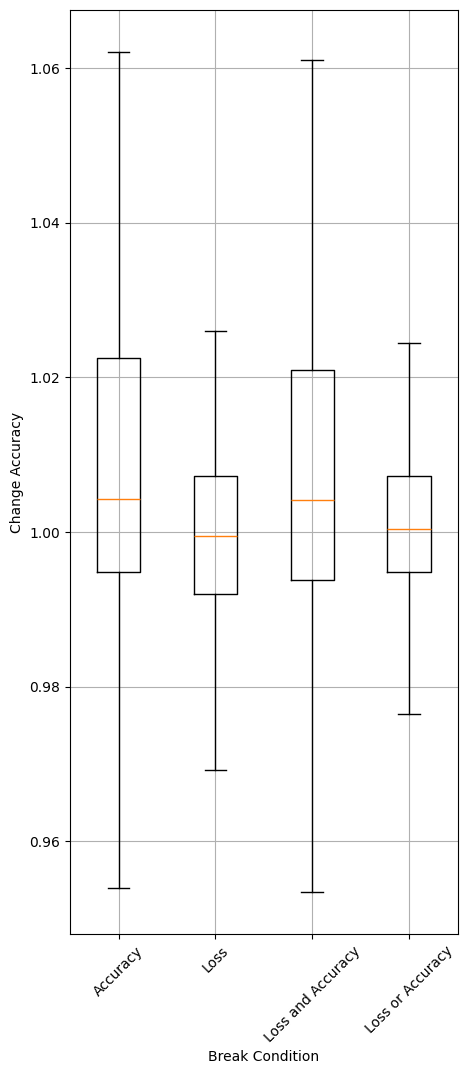
\includegraphics[width=0.95\textwidth]{plots/BreakCondition_NotTrained_accuracy.png}
    \end{subfigure}
    \begin{subfigure}{0.5\textwidth}
        \centering
        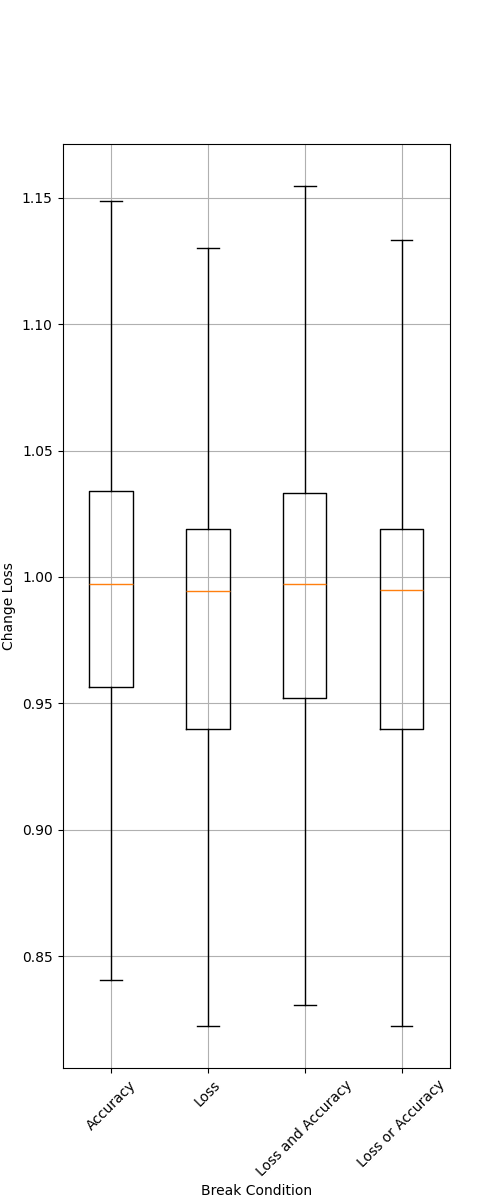
\includegraphics[width=0.95\textwidth]{plots/BreakCondition_NotTrained_loss.png}
    \end{subfigure}
    \caption{Loss and accuracy, without training, with different break conditions}
    \label{fig:break-conditions-notraining}
\end{figure}
\subsection{Contributions of Different Mutation Functions}\label{subsec:contributions-of-different-mutation-functions}
There were no significant differences between the functions examined for the trained runs \ref{fig:mutation-functions-training}, except for \texttt{modify\_weight\_all\_random\_by\_scalar\_gauss} \ref{lst:scalar_weight_mod}, which performed worse in terms of both loss and accuracy.
In contrast, the non-trained \ref{fig:mutation-functions-notraining} runs yielded similar results for the weight modifying functions, but no significant improvements were observed when using bias modifying functions.
\begin{figure}
    \begin{subfigure}{0.5\textwidth}
        \centering
        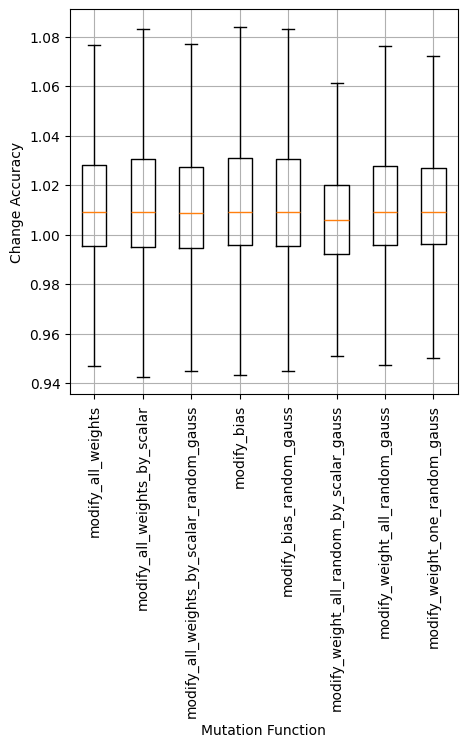
\includegraphics[width=0.95\textwidth]{plots/Mutatation_Trained_accuracy.png}
    \end{subfigure}
    \begin{subfigure}{0.5\textwidth}
        \centering
        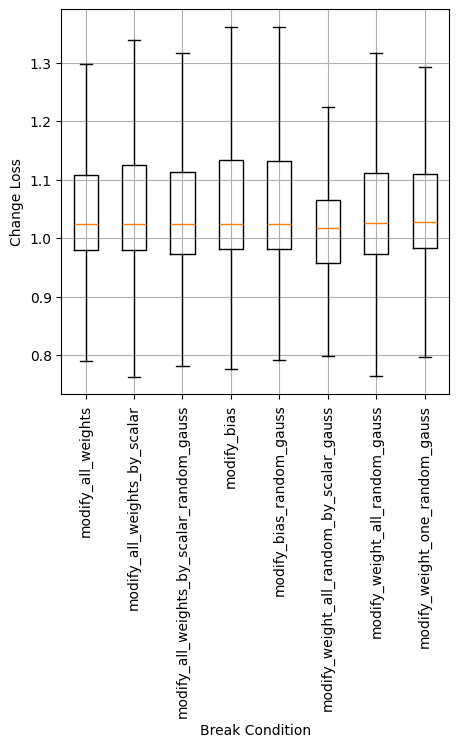
\includegraphics[width=0.95\textwidth]{plots/Mutatation_Trained_loss.png}
    \end{subfigure}
    \caption{Loss and accuracy, with training, with different mutation functions}
    \label{fig:mutation-functions-training}
\end{figure}
\begin{figure}
    \begin{subfigure}{0.5\textwidth}
        \centering
        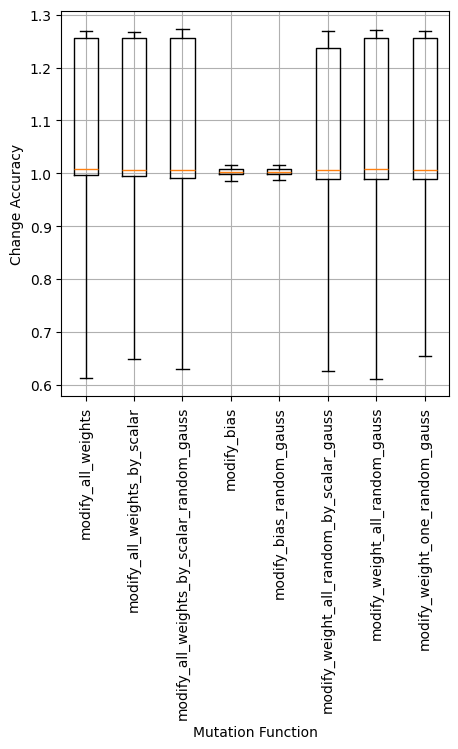
\includegraphics[width=0.95\textwidth]{plots/Mutatation_NotTrained_accuracy.png}
    \end{subfigure}
    \begin{subfigure}{0.5\textwidth}
        \centering
        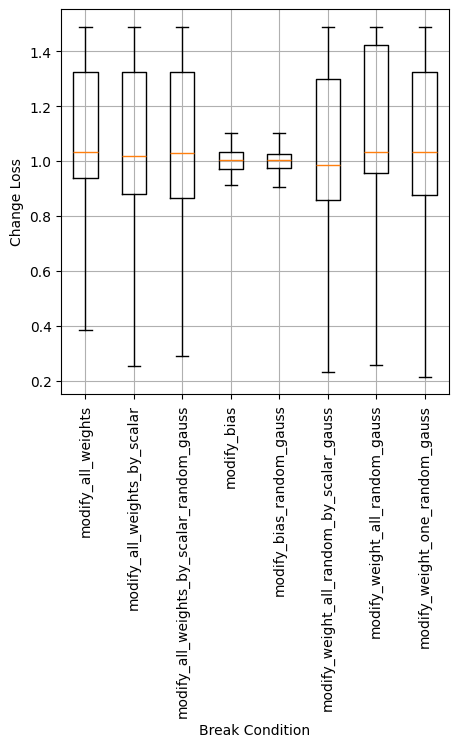
\includegraphics[width=0.95\textwidth]{plots/Mutatation_NotTrained_loss.png}
    \end{subfigure}
    \caption{Loss and accuracy, without training, with different mutation functions}
    \label{fig:mutation-functions-notraining}
\end{figure}
In regard to the values we are using for the mutation functions, there is no significant difference between the different values for the trained runs \ref{fig:mutation-values-training} or the untrained runs \ref{fig:mutation-values-notraining}.
\begin{figure}
    \begin{subfigure}{0.5\textwidth}
        \centering
        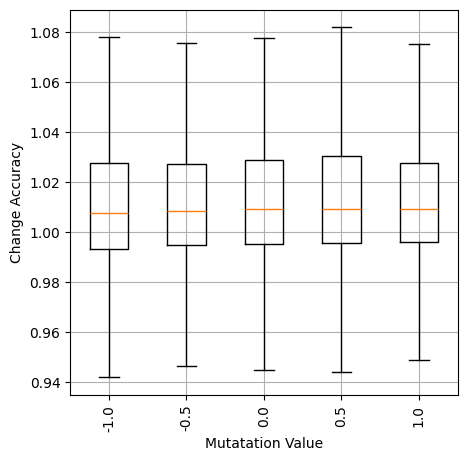
\includegraphics[width=0.95\textwidth]{plots/MutatationValue_Trained_accuracy.png}
    \end{subfigure}
    \begin{subfigure}{0.5\textwidth}
        \centering
        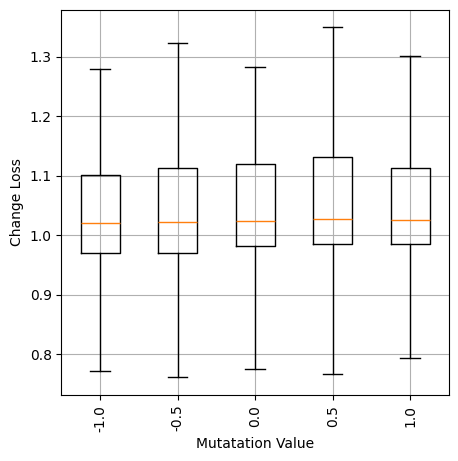
\includegraphics[width=0.95\textwidth]{plots/MutatationValue_Trained_loss.png}
    \end{subfigure}
    \caption{Loss and accuracy, with training, with different mutation values}
    \label{fig:mutation-values-training}
\end{figure}
\begin{figure}
    \begin{subfigure}{0.5\textwidth}
        \centering
        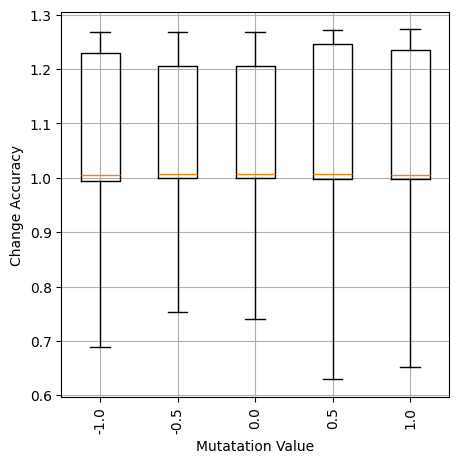
\includegraphics[width=0.95\textwidth]{plots/MutatationValue_NotTrained_accuracy.png}
    \end{subfigure}
    \begin{subfigure}{0.5\textwidth}
        \centering
        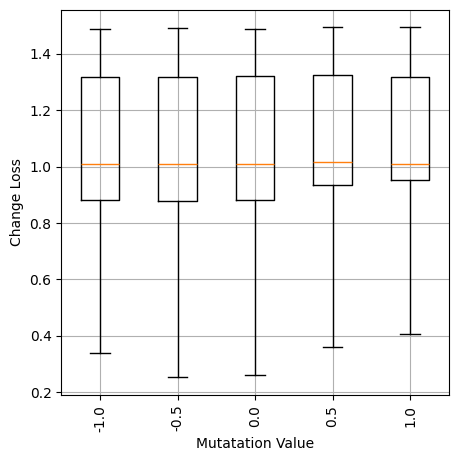
\includegraphics[width=0.95\textwidth]{plots/MutatationValue_NotTrained_loss.png}
    \end{subfigure}
    \caption{Loss and accuracy, without training, with different mutation values}
    \label{fig:mutation-values-notraining}
\end{figure}
